Once jet objects are reconstructed, they undergo a series of calibrations to correct for the various inputs, as well as contributions from non-interacting particles such as neutrinos. The jet energy calibration consists of a six-stage process with a schematic of this seen in Figure~\ref{fig:reco_jets_calibration_stream}.

\begin{figure}[htp]
  \centering
  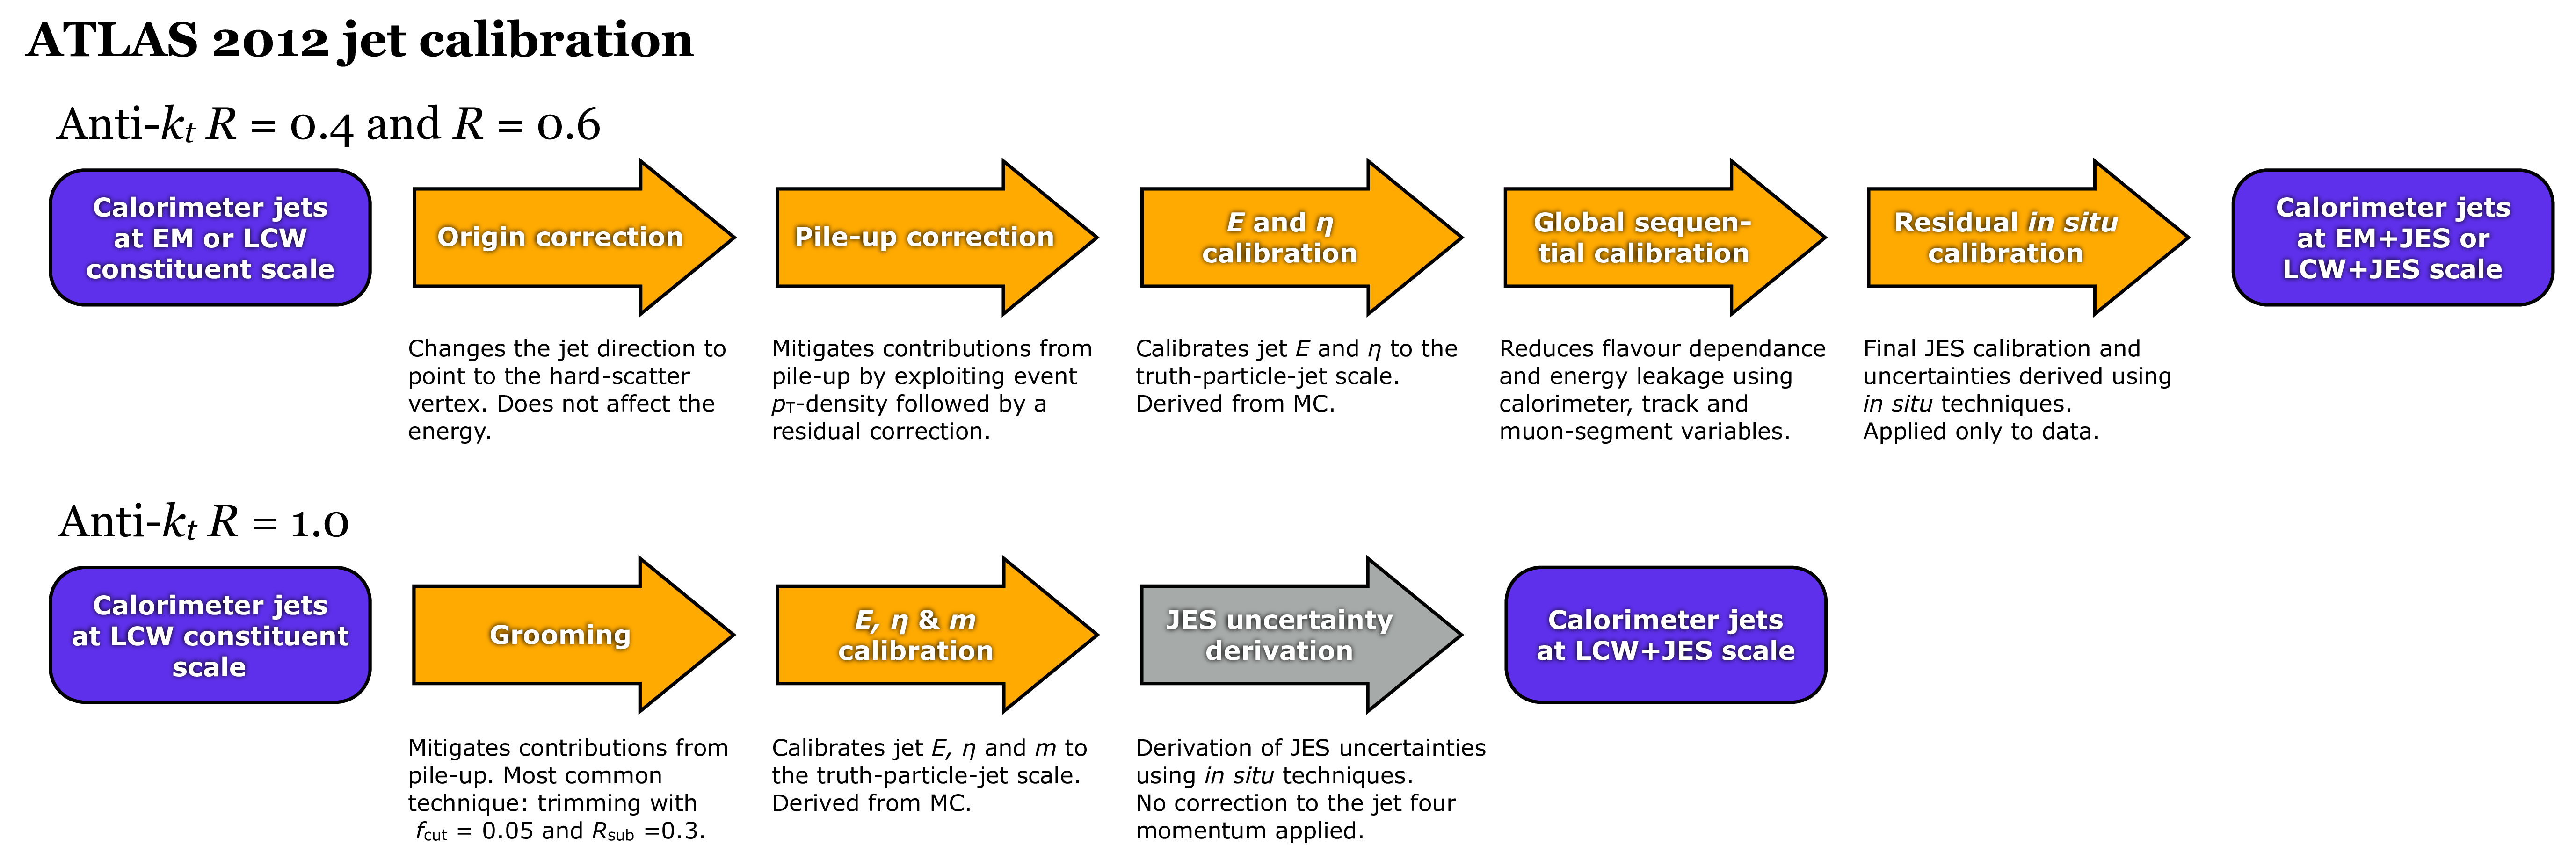
\includegraphics[width=1\textwidth]{figures/reco/reco_jet_calibration_stream.png}
  \caption{Illustration of the ATLAS jet calibration. Taken from Ref.~\cite{ATLAS:2019oxp}.}\label{fig:reco_jets_calibration_stream}
\end{figure}

The process begins by adjusting the jet's direction to point back to the PV by altering the jet's 4 vector such that the energy remains unchanged. Then, the impact of pile-up is mitigated using an area-based subtraction method, as detailed in Ref.~\cite{ATLAS:2013eua}. Following these, the jet energy is calibrated using the jet energy scale (JES), which is a correction factor derived from MC simulations relating jet energy to the energy of the corresponding truth-level jet. Additional corrections are also applied to account for different detector responses between quark- and gluon-initiated jets, as well as for jets that are only partially contained within the calorimeter. The final step involves jet energy resolution (JER) calibration which is performed by comparing data and MC simulation and can be read in detail in Ref.~\cite{ATLAS:2019oxp}. 